\part{Tutorials}
	\section{Quick Start}
		This is a quick start guide for the Kerbal Operating System (kOS). It is intended for those who are just starting with using kOS. It does presume you have played Kerbal Space Program before and know the basics of how to fly a rocket under manual control. It does NOT assume you know a lot about computer programming, and it will walk you through some basic first steps.
		First example: Hello World
In the grand tradition of programming tutorials, the first example will be how to make a script that does nothing more than print the words ?Hello World? on the screen. The purpose of this example is to show where you should put the files, how to move them about, and how to get one to run on the vessel.

Step 1: Start a new sandbox-mode game
(You can use kOS in a career mode game, but it requires a part that you have to research which isn?t available at the start of the tech tree, so this example will just use sandbox mode to keep it simple.)

Step 2: Make a vessel in the Vehicle Assembly Bay
Make the vessel contain any unmanned command core, a few hundred units of battery power, a means of recharging the battery such as a solar panel array, and the ?Comptronix CX-4181 Scriptable Control System?. (From this point onward the CX-4181 Scriptable Control System part will be referred to by the acronym ?SCS?.) The SCS part is located in the parts bin under the ?Control? tab (the same place where RCS thrusters and Torque Wheels are found.)

\begin{center}
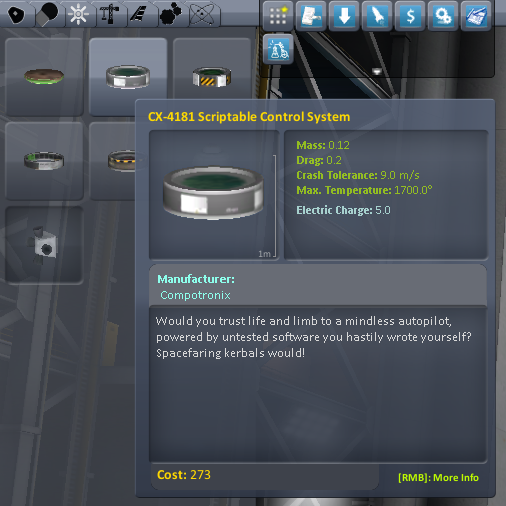
\includegraphics[width=3in]{SCS_parts_bin}
\end{center}

Step 3: Put the vessel on the launchpad
Put the vessel on the launchpad. For this first example it doesn?t matter if the vessel can actually liftoff or even has engines at all.

Step 4: Invoke the terminal
Rightclick for the SCS part on the vessel and then click the button that says ?Open Terminal?.

Note that if the terminal is semi-transparent, this means it?s not currently selected. If you click on the terminal, then your keyboard input is directed to the terminal INSTEAD of to piloting. In other words if you type W A S D, you?ll actually get the word ?wasd? to appear on the terminal, rather than the W A S D keys steering the ship. To switch back to manual control of the game instead of typing into the terminal, click outside the terminal window anywhere on the background of the screen.

Step 5: See what an interactive command is like
You should now see an old-school looking text terminal like the one shown below. Type the line:

CLEARSCREEN. PRINT "==HELLO WORLD==".
into the terminal (make sure to actually type the periods (?.?) as shown) and hit ENTER. Note that you can type it in uppercase or lowercase. kOS doesn?t care.

\begin{center}
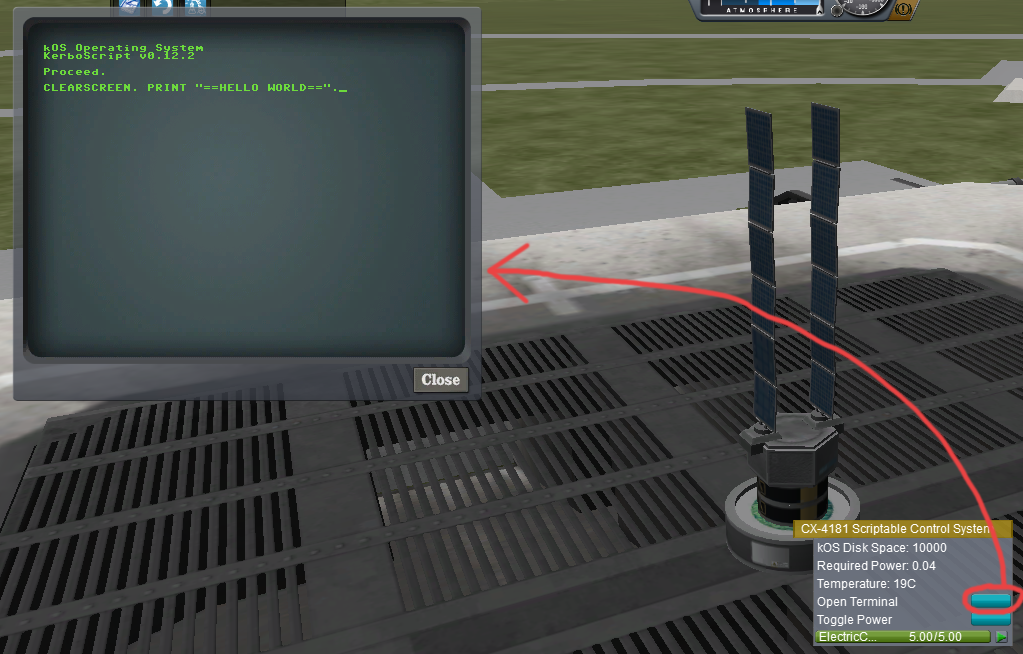
\includegraphics[width=3in]{terminal_open_1}
\end{center}

The terminal will respond by showing you this:

\begin{center}
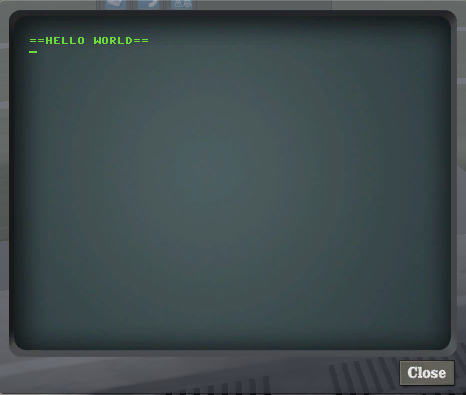
\includegraphics[width=3in]{terminal_open_2}
\end{center}

Step 6: Okay that?s great, but how can you make that happen in a program script instead?
Like so: Enter this command:

EDIT HELLO.
(Don?t forget the period (?.?). All commands in kOS are ended with a period. Again, you can type it in uppercase or lowercase. kOS doesn?t care.)

You should see an editor window appear, looking something like this (without the text inside because you?re starting a blank new file):

\begin{center}
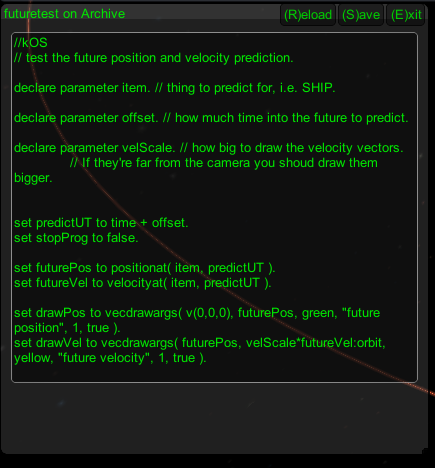
\includegraphics[width=3in]{editor}
\end{center}

Type this text into the window:

PRINT "=========================================".
PRINT "      HELLO WORLD".
PRINT "THIS IS THE FIRST SCRIPT I WROTE IN kOS.".
PRINT "=========================================".
Click ?Save? then ?Exit? in the editor popup window.

Side Note: The editor font - Experienced programmers may have noticed that the editor?s font is proportional width rather than monospaced and that this is not ideal for programming work. You are right, but there is little that can be done about it for a variety of technical reasons that are too complex to go into right now.
Then on the main text terminal Enter:

RUN HELLO.
And you will see the program run, showing the text on the screen like so.

\begin{center}
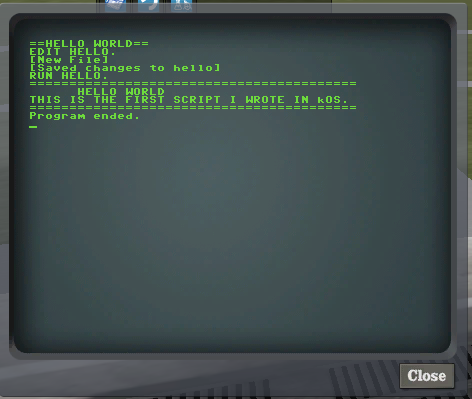
\includegraphics[width=3in]{hello_world1}
\end{center}

Step 7: Okay, but where is this program?
To see where the ?HELLO? program has been saved, Issue the command LIST FILES like this:

LIST FILES.
(Note, that the default for the LIST command is to list FILES, so you can leave the word ?FILES? off if you like.)

It should look like this, showing you the HELLO program you just wrote:

\begin{center}
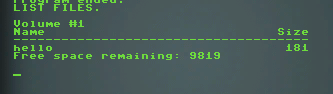
\includegraphics[width=3in]{hello_list.png}
\end{center}

This is a list of all the files on the currently selected VOLUME. By default, when you launch a new vessel, the currently selected VOLUME is called ?1? and it?s the volume that?s stored on THAT SCS part that you are running all these commands in.

This is the local volume of that SCS part. Local volumes such at this tend to have very small limited storage, as you can see when you look at the space remaining in the list printout.

If you?re wondering where the file is stored physically on your computer, it?s represented by a section inside the persistence file for your saved game, as a piece of data associated with the SCS part. This is important because it means you can?t access the program from another vessel, and if this vessel ever crashes and the SCS part explodes, then you?ve lost the program.

Step 8: I don?t like the idea that the program is stored only on this vessel. Can?t I save it somewhere better? More permanent?
Yes. Yes you can.

There is another VOLUME that always exists called the Archive, which is also referred to as volume 0. (either name can be used in commands). The archive is conceptually stored somewhere back at Kerbin home base in the Space Center rather than on your vessel. It has infinite storage space, and does not disappear when your vessel is gone. ALSO, it actually exists across saved games - if you launch one saved game, put a new file in the Archive, and then later launch a different saved game, that file will be there in that game too.

To use the Archive, first we?ll have to introduce you to a new command, called SWITCH TO. The SWITCH TO command changes which VOLUME is the one that you are doing your work with.

To work with the archive, and create a second ?hello world? file there, you issue these commands and see what they do:

SWITCH TO 0.
EDIT HELLO2. // Make a new file here that just says: PRINT "hi again".
LIST FILES.
RUN HELLO2.
SWITCH TO 1.
LIST FILES.
RUN HELLO.
But where is it stored behind the scenes? The archive is currently slightly violating the design of KSP mods that puts everything in the GameData folder. The kSP Archive is actually stored in the Ships/Script folder of your MAIN KSP home, not inside GameData.

If a file is stored inside the archive, it can actually be edited by an external text editor of your choice instead of using kOS?s in-game editor. This is usually a much better practice once you start doing more complex things with kOS. You can also make new files in the archive folder. Just make sure that all the files end with a .ks file name suffix or kOS won?t use them.	

Further reading about files and volumes:

Volumes
File Control
File Information		
	\section{Design Patterns}
	\section{PID Loops}
	\section{Execute Node Script}